
When quench propagates, the point at which the cable transitions from superconducting to the normal conducting state propagates with time, as shown in Fig. \ref{fig:quench_front_propagation_illustration}. This point remains at the critical temperature, $T_\text{c}$ for a given magnetic field strength. Its time derivative is referred to as quench velocity. Depending on electro-magneto-thermal conditions at which quench occurs, quench velocity can remain constant or change in time. 

\begin{figure}[H]
\centering
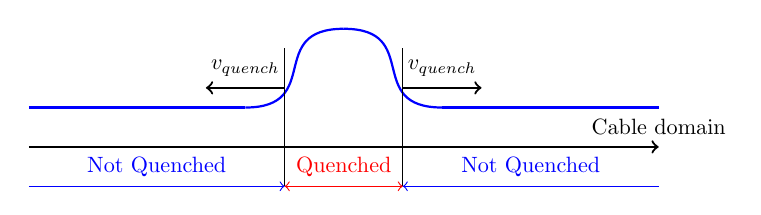
\begin{tikzpicture}[scale = 1]
\draw [thick, ->] (0.0,0.0) -- (8.0,0);

\draw [thick, blue] (0.0,0.5) -- (2.75,0.5);
\draw [thick, blue] (5.25,0.5) -- (8.0,0.5);

\draw [thick, blue] (2.75,0.5) .. controls +(0:1cm) and +(180:1cm) .. (4.0,1.5);
\draw [thick, blue] (4.0,1.5) .. controls +(0:1cm) and +(180:1cm) .. (5.25,0.5);

\draw [thin] (3.25,-0.5) -- (3.25,1.25);
\draw [thin] (4.75,-0.5) -- (4.75,1.25);

\draw [thick, ->] (4.75,0.75) -- (5.75,0.75);
\draw [thick, ->] (3.25,0.75) -- (2.25,0.75);

\draw [thin, red, <->] (3.25,-0.5) -- (4.75,-0.5);
\draw [thin, blue, ->] (0.0,-0.5) -- (3.25,-0.5);
\draw [thin, blue, <-] (4.75,-0.5) -- (8.0,-0.5);

\node[scale = 0.8] [color = red] at (4.0,-0.25) {Quenched};
\node[scale = 0.8] [color = blue] at (1.625,-0.25) {Not Quenched};
\node[scale = 0.8] [color = blue] at (6.375,-0.25) {Not Quenched};

\node[scale = 0.8] at (5.25,1.0) {$v_\text{quench}$};
\node[scale = 0.8] at (2.75,1.0) {$v_\text{quench}$};
\node[scale = 0.8] at (8.0,+0.25) {Cable domain};

\end{tikzpicture}
\caption{Quench velocity approach.}
\label{fig:quench_front_propagation_illustration}
\end{figure}

Quench velocity can be approximated with analytic formulae. They are usually a function of current density, composite strand material properties and temperature gradient around the quench front. The quench velocity in ITER applications is mainly estimated based on~\cite{MIT_phd_thesis}. For superconducting accelerator magnets, Wilson's formula is more applicable if cooling with helium is not considered \cite[p.~206]{wilson1987superconducting}. In general, quench velocity can be estimated in three different manners. It can be:
\begin{enumerate}
\item based on available measurements,
\item calculated analytically based on available formulae,
\item calculated numerically based on short numerical model with refined mesh to solve the quench front with sufficient precision.
\end{enumerate}